\documentclass[a4paper]{article}
\usepackage[usenames,dvipsnames]{xcolor}
\usepackage{caption}
\usepackage{amsmath}
\usepackage{amsfonts}
\usepackage{amssymb}
\usepackage{subcaption}
\usepackage{listings}
\usepackage{qtree}
\usepackage{xcolor}
\usepackage{forest}
\usepackage{multicol}
\setlength{\columnsep}{3cm}
\usepackage{parskip}
\usepackage{changepage}
\usepackage[T1]{fontenc}
\usepackage{amsmath}
\usepackage{hyperref}
\usepackage{listings}
\usepackage{amsthm}
\usepackage{amssymb}
\usepackage{float}
\usepackage[utf8]{inputenc}
\usepackage{graphicx}
\usepackage[italian]{babel}
\usepackage{thmtools}
\usepackage{mathtools}
\newtheorem*{definition}{Def}
\usepackage{xcolor}
\newcommand{\appunto}[1]{\textcolor{ForestGreen}{#1}}
\newcommand{\E}[0]{\mathbb{E}}
\renewcommand{\thesubsection}{\thesection.\alph{subsection}}


\begin{document}

\author{Giulia Coucorde 802321 giulia.coucourde@edu.unito.it,\\ Andrea Cacioli 914501 andrea.cacioli@edu.unito.it,\\ Lorenzo Dentis 914833 lorenzo.dentis@edu.unito.it}
\title{Risposte Foglio1}
\maketitle
\section{Esercizio 1}
Si consideri una catena di Markov con matrice di transizione.
$$P=\left(\begin{array}{c c c}{{\frac{1}{2}}}&{{\frac{1}{3}}}&{{\frac{1}{4}}}\\ {{\frac{3}{4}}}&{{0}}&{{\frac{1}{4}}}\\ {{0}}&{{1}}&{{0}}\end{array}\right)$$
\begin{itemize}
	\item Stabilire se sia una catena irreducibile.\\
	Una catena si dice irreducibile quando presenta una sola classe di equivalenza rispetto alla relazione \textit{comunicazione}.
		Si dimostra facilmente che $P$ è irreducibile disegnando il suo grafo pesato:\\
		\begin{center}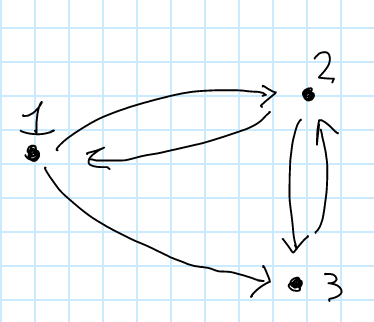
\includegraphics[scale=0.3]{grafo.png}\end{center}
		Dal disegno si nota facilmente che ${1,2,3}$ è l'unica classe di equivalenza della catena, $(1,2)$ e $(2,3)$ comunicano direttamente, la coppia $(1,3)$ comunica grazie alla transitività della relazione \textit{comunicazione}.\\
		$ 1 \rightarrow 3$ è una relazione di comunicazione diretta e $3 \rightarrow 2 \land 2 \rightarrow 1 \Rightarrow 3 \rightarrow 1$ 
	\item Supponendo che il processo sia originato nello stato 1, determinare la probabilitá che si trovi nello stato 3 dopo due passi\\
		Per trovare la probabilità che un sistema si trovi in un dato stato basta utilizzare la matrice di transizione, come dimostrato a lezione se si vuole considerare l'evoluzione dopo $n$ passi basta considerare la matrice di transizione $P^n$. In questo caso ci interessa $P^2$.\\
		$$P^2=P*P= \left(\begin{array}{c c c}{{\frac{1}{2}}}&{{\frac{1}{3}}}&{{\frac{1}{4}}}\\ {{\frac{3}{4}}}&{{0}}&{{\frac{1}{4}}}\\ {{0}}&{{1}}&{{0}}\end{array}\right) *
		\left(\begin{array}{c c c}{{\frac{1}{2}}}&{{\frac{1}{3}}}&{{\frac{1}{4}}}\\ {{\frac{3}{4}}}&{{0}}&{{\frac{1}{4}}}\\ {{0}}&{{1}}&{{0}}\end{array}\right)
		= \left(\begin{array}{c c c}{{\frac{1}{2}}}&{{\frac{1}{3}}}&{{\frac{1}{6}}}\\ {{\frac{3}{8}}}&{{\frac{1}{2}}}&{{\frac{1}{8}}}\\ {{\frac{3}{4}}}&{{0}}&{{\frac{1}{4}}}\end{array}\right) $$
	\item Determinare $lim_{n \rightarrow \infty}P^n$
		Per ottenere la distribuzione limite possiamo utilizzare il teorema presentato in classe. La catena $P$ è irreducibile (dimostrato al punto 1) ed Ergodica, questo perchè tutti gli stati sono aperiodici e la catena è irreducibile, quindi sappiamo:
		\begin{enumerate}
			\item esiste $lim_{n\rightarrow\infty}P^n_{ij}=\Pi_j$
			\item $\Pi_j$ è l'unica soluzione del seguente sistema: 
				\begin{equation*}
					\begin{cases} \Pi_j = \sum_i \Pi_j P_{ij}\\
						\sum \Pi_j = 1
					\end{cases}
				\end{equation*}
		\end{enumerate}
		Aplicandolo al nostro caso ottieniamo il seguente sistema:
		\begin{align*}
			\begin{cases}
				\frac{1}{2}\Pi_1 * \frac{3}{4}\Pi_2 * 0\Pi_3 = \Pi\\
				\frac{1}{3}\Pi_1 * 0\Pi_2 * 1\Pi_3 = \Pi\\
				\frac{1}{6}\Pi_1 * \frac{1}{4}\Pi_2 * 0\Pi_3 = \Pi\\
				\Pi_1 + \Pi_2 + \Pi_3 = 1
			\end{cases}
			= \textit{ risolvendo } = 
			\begin{cases}
				\Pi_1 = \frac{1}{2}\\
				\Pi_2 = \frac{1}{3}\\
				\Pi_3 = \frac{1}{6}
			\end{cases}
		\end{align*}
\end{itemize}
\section{Esercizio 3}
Si considerino due processi di Poisson, indipendenti $N_1(t)$ e $ N_2(t)$ di parametri $\mu_1$ e $\mu_2$ , rispettivamente.
\subsection{}
Si determini la distribuzione degli intertempi del processo $M (t) = N_1 (t) + N_2 (t)$
Siano $E_1$ ed $E_2$ gli intertempi rispettivamente del processo $M_1$ ed $M_2$.\\
L' unico modo per ottenere un intertempo di $M$ di durata $\leq x$ è che $E_1 \leq x \wedge E_2 \geq x$ oppure $E_2 \leq x \wedge E_1 \geq x$.
Per cui la distribuzione di $E$ (intertempo di $M$) è:
\begin{align*}
	P(E \leq x) =& P(E_1 \leq x) P(E_2 \geq x) + P(E_1 \leq x)P(E_2 \geq x)=\\
	=&2 * (1-e^{-\lambda x}) * e^{-\lambda x}=\\
	=& 2 * (e^{-\lambda x} - e^{-2\lambda x})
\end{align*}

\subsection{}
Determinare la distribuzione condizionale di $N_1 (t)$ dato $ M (t) = 1$
$$P(N_1 = 1 | M = 1) = P (N_1 = 1 | N_1 + N_2 = 1)$$
Le condizioni necessarie per cui questo si verifichi sono le seguenti:
$$N_1 = 1 \wedge N_2 = 0$$
ma 
$$N_1 ~ Pois(\mu_1) \qquad N_2 ~ Pois(\mu_2)$$
per indipendenza delle due distribuzioni:
\begin{align*}
	&P(N_1 = 1) * P(N_2 = 0) = \\
	&\frac{\mu_1^1}{1!}*e^{-\mu_1}\frac{\mu_2^0}{0!}*e^{-\mu_2}=\\
	&= \mu_1*e^{-\mu_1}e^{-\mu_2}= \mu_1*e^{-\mu_1-\mu_2}
\end{align*}

\subsection{}
Si suggerisca un metodo per simulare una traiettoria di $M (t)$ fino al tempo $ t = 10$ avendo giá a disposizione la simulazione di una traiettoria di $ N1 (t) $ fino al tempo $ t = 11$\\

Simulo variabili aleatorie esponenziali di parametro {{aspetta la risposta della prof}} finché la somma di tutte é $\leq 10$.
A questo punto ho una traccia di $N_2$ fino a 10 e la sommo con la traccia fornitami di $N_1$ fino a 10.
In questo modo ho una possibile traccia di $M$.

\section{Esercizio 3}
Sei schermi vengono controllati simultaneamente. Ciascuno ha una durata in vita esponenziale di parametri $\lambda_i , i = 1, .., 6$, indipendentemente uno dall’altro
\subsection{}
Quanto tempo si deve attendere prima che se ne guasti uno? Si fornisca la distribuzione e il suo valore atteso. Quanto tempo si deve attendere prima che ce ne siano 2 guasti? Si fornisca la distribuzione e il suo valore atteso.
Possiamo considerare i tempi prima che un teleschermo si rompa come degli intertempi del processo di Poisson che conta il numero di rotture nel sistema dei teleschermi.
Siccome siamo in un processo di Poisson, gli intertempi sono esponenziali indipendenti
Per trovare il minimo in un insieme di esponenziali indipendenti identicamente distribuiti uso la seguente formula:
$$min\{exp_i\}= \frac{\lambda}{n \lambda}$$
Ma non essendo identicamente distribuiti, la formula diventa:
$$min\{exp_i\}= \frac{\lambda_{min}}{\sum_1^n \lambda_i}$$

Per trovare il secondo minimo utilizzo la stessa formula ma con al numeratore:  
$$min(\{exp_i\}\setminus \{\lambda_{min}\}) $$
\subsection{}
Quanto tempo si deve attendere prima che si rompano tutti? Si fornisca la distribuzione e il valore atteso.\\

La probabilità che tutti si siano rotti è equivalente a trovare la probabilità che l'ultimo si sia rotto (quello con il tempo più alto di tutti), quindi:
$$min\{exp_i\}= \frac{\lambda_{max}}{\sum_1^n \lambda_i}$$



\section{Esercizio 4}
Si considerino due distinte code di tipo M/M/1 (code in cui i clienti arrivino secondo un processo di Poisson e vengano serviti da un unico servitore con tempi di servizio esponenziali).
Si supponga che nella prima coda il processo di Poisson abbia parametro $\lambda_1$ , mentre nella seconda abbia parametro $\lambda_2$ ; inoltre il tempo di servizio sia analogo per le due code, con tempo medio di servizio $\mu$. Si supponga $\lambda_1 < \lambda_2 < \mu$
\subsection{}
Si puó affermare che in ogni istante ci saranno sicuramente meno clienti in attesa nella prima coda?
No, non lo si può affermare, in quanto si possono trovare 3 controesempi:\\
Il primo controesempio è la situazione in cui non c'è alcun cliente in coda ed arriva un cliente prima prima coda che nella seconda, cosa comunque possibile nonostante $\lambda_1 < \lambda_2$.\\
Più interessante è la situazione in cui entrambe le code hanno $n$ clienti. 
\begin{center}\makebox[0cm]{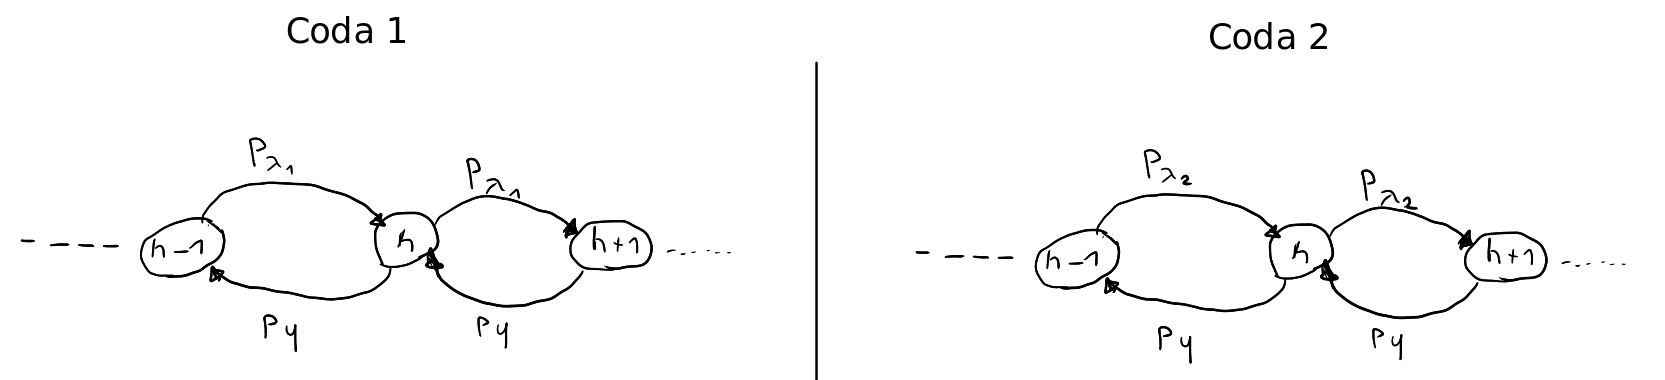
\includegraphics[scale=0.3]{code.png}}\end{center}
In questo caso ci sono due situazioni in cui la prima coda ha più clienti in attesa della seconda, se un cliente arriva nella coda 1 ($P_{\lambda_1}$), o se un cliente esce dalla coda 2 ($P_\mu$).
\subsection{}
Si puó affermare che in media ci saranno meno clienti nella coda 1? Giustificare la risposta.
Si, in media ci saranno meno clienti nella prima coda. Tra le proprietà della coda M|M|1 vi è una proprietà che, sotto la condizione $\lambda < \mu$, permette di calcolare il numero medio di persone in coda.
\begin{align*}
	&\text{posto } \lambda < \mu \text{ e creando un nuovo parametro } \rho = \frac{\lambda}{\mu} \\
	&\text{Il numero medio di utenti in coda è } L_{q}=\sum_{k=1}^{\infty}{(k-1)\pi_{i}}=\frac{\rho^{2}}{1-\rho}
\end{align*}
Nel caso dell'esercizio $\lambda_1 < \lambda_2$ e $\mu$ uguale per le due code quindi\\ $\rho_1 = \frac{\lambda_1}{\mu} < \rho_2 = \frac{\lambda_2}{\mu}$
$$L_{q1} = \frac{\rho_1^{2}}{1-\rho_1} < L_{q2} = \frac{\rho_2^{2}}{1-\rho_2}$$
Si può quindi affermare che in media la coda 2 avrà più clienti della coda 1.
\end{document}
